\documentclass[ignorenonframetext,t,10pt]{beamer}

\mode<presentation>
{ \usetheme{boxes} }


\usetheme[hideothersubsections]{UNLTheme}

%\usetheme{Warsaw}
%\usecolortheme{default}
%\useoutertheme{split}
%\useinnertheme{rectangles}
\definecolor{beamer@lblue}{rgb}{0.5,0.5,0.9}
\definecolor{beamer@dblue}{rgb}{0.1,0.1,0.5}
\setbeamercolor{structure}{fg=beamer@dblue}
%\beamertemplatenavigationsymbolsempty

% Language packages
\usepackage[english]{babel}
\usepackage[utf8]{inputenc}

% Packages
%%%%%%%%%%%%%%%%%%%%%%%%%%%%%%
% AMS packages
\usepackage{amsthm}
\usepackage{amsmath}
\usepackage{amsfonts}

% Images/figures
\usepackage{graphicx}
\usepackage{subfigure}

% Other
\usepackage{verbatim}
\usepackage{ifthen}
\usepackage{algorithmic}

\usepackage{epstopdf}

\usepackage{graphicx} %The mode "LaTeX => PDF" allows the following formats: .jpg  .png  .pdf  .mps
%\usepackage{media9}
\usepackage{movie15}

\usepackage{tikz}
\usetikzlibrary{shapes,arrows}

%%%%%%%%%%%%%%%%%%%%%%%%%%%%%%%

% Define some useful colors
\definecolor{tannerBlue}{rgb}{0.255,0.41,0.884} % RoyalBlue
\definecolor{tannerRed}{rgb}{1,0,0} % Red
% to use these colors: \textcolor{tannerBlue}{this text is blue}

% Commands
\newcommand{\tpvspace}{\vspace{5pt}}
\newcommand{\nicesum}{\displaystyle \sum}

%the following commands are used to align and insert slide numbers
\newcommand{\numspace}
{
  \ifthenelse{\insertframenumber < 10}{\hspace{30pt}}{\hspace{32pt}}
}
%\newcommand{\framenumbers}{\numspace\insertframenumber/{9}}

\newcommand{\pdfmovie}[4]{\href{run:#1}{\framebox{\parbox[c][#3][c]{#2}{\center #4}}}}


\pgfdeclareimage[height=1.0cm]{logo}{plots/Harvard}
\logo{\pgfuseimage{logo}}

% Title
\title[Limiting the effects of earthquakes on gravitational-wave interferometers]{Limiting the effects of earthquakes on gravitational-wave interferometers}
\author[M.~Coughlin]{Nicolas Arnaud, David Barker, Sebastien Biscans, Christopher Buchanan, Eric Coughlin, Michael Coughlin, Fred Donovan, Paul S Earle, Jeremy Fee, Hunter Gabbard, Jan Harms, Irene Fiori, Michelle R Guy, Nikhil Mukund, Matthew Robert Perry, Hugh Radkins, Bas Swinkels, Keith Thorne, Jim Warner}
\date[]{March 14, 2017}

\begin{document}

\maketitle

\begin{frame}
\titlepage
\end{frame}

\section{Introduction}

\begin{frame}
\frametitle{Introduction}

  \begin{enumerate}
  \item The detectors are susceptible to teleseismic events, which can significantly impact a detector's duty cycle. 
  \item Here we describe an early-warning system for gravitational-wave observatories, which relies on near real-time earthquake alerts provided by the U.S. Geological Survey (USGS) and the National Oceanic and Atmospheric Administration (NOAA).
  \item Our initial results indicate that by using detector control configuration changes, we could regain duty cycle otherwise lost during earthquake events.
  \end{enumerate}
\end{frame}

\section{Algorithm}

\begin{frame}
\frametitle{Pipeline}

% Define block styles
\tikzstyle{decision} = [diamond, draw, fill=blue!20,
    text width=4.5em, text badly centered, node distance=3cm, inner sep=0pt]
\tikzstyle{block} = [rectangle, draw, fill=blue!20,
    text width=5em, text centered, rounded corners, minimum height=3em]
\tikzstyle{line} = [draw, -latex']
\tikzstyle{cloud} = [draw, ellipse,fill=red!20, node distance=3cm,
    minimum height=2em]
\tikzstyle{emptyblock} = [rectangle, minimum height=3em]

\begin{figure}[t]
 \begin{center}
 \begin{tikzpicture}[node distance = 1.5cm, auto]
    % Place nodes
    \node [emptyblock] (init) {};
    \node [block, left of=init] (PDL) {PDL};
    \node [block, right of=init] (GeoJSON) {GeoJSON};
    \node [block, below of=init] (Parse) {Parse events};
    \node [block, below of=Parse] (Traveltimes) {Calculate travel times};
    \node [block, below of=Traveltimes] (XML) {Produce XML files};
    \node [block, below of=PDL, node distance=6cm] (Plot) {Summary / Plot};
    \node [block, below of=GeoJSON, node distance=6cm] (Epics) {Site Notification};
    % Draw edges
    \path [line] (PDL) -- (Parse);
    \path [line] (GeoJSON) -- (Parse);
    \path [line] (Parse) -- (Traveltimes);
    \path [line] (Traveltimes) -- (XML);
    \path [line] (XML) -- (Plot);
    \path [line] (XML) -- (Epics);
 \end{tikzpicture}
 \end{center}
 \caption{A flow chart of the \emph{Seismon} pipeline. The USGS's Product Distribution Layer (PDL) and public GeoJSON earthquake files provide information used by \emph{Seismon} to compute estimated site arrival times and Rayleigh wave velocities.}
 \label{fig:flowchart}
\end{figure}
\end{frame}

\begin{frame}
\frametitle{Notices}

  \begin{enumerate}
\item Warning system relies on the most preliminary notices of earthquakes currently available generated by worldwide networks of seismometers. 
\item USGS provides preliminary estimates of the location providing latitude, longitude, and depth of each event.
\item These solutions are distributed through USGS's Product Distribution Layer (PDL), which has been configured to receive notifications for all located earthquakes worldwide. 
  \end{enumerate}
\end{frame}

\begin{frame}
\frametitle{Site Notification}

  \begin{enumerate}
\item We use the ground velocity at the site and time-of-arrival predictions to create warnings for the detectors.
\item The algorithm analyzes the recent notifications and places a threshold on the predictions.
\item We provide a set of variables that contains the following information: amplitude prediction, probability of lockloss, earthquake time-of-arrival.
  \end{enumerate}
  
We estimate the amplitude of the surface waves, $\rm Rf_{amp}$, at the sites using the equation
\begin{equation}
{\rm Rf_{amp}} = M \frac{\rm a}{f_c^{b}} \frac{e^{-2 \pi h f_{\rm c}/c}}{r^{d}}
\label{eq:Rfamp} 
\end{equation}
where $f_{\rm c} = 10^{2.3-M/2}\,\rm$ is the corner frequency of the earthquake,  $M$ is the magnitude of the earthquake, $h$ is the depth, $r$ is the distance to the detectors, and $c$ is the speed of the surface-waves, all in SI units.  
  
\end{frame}

\begin{frame}
  \frametitle{Comparison of initial versus final magnitude estimates}
\begin{center}
\begin{figure}[hbtp!]
  \subfigure[Comparison of initial versus final magnitude estimates.]{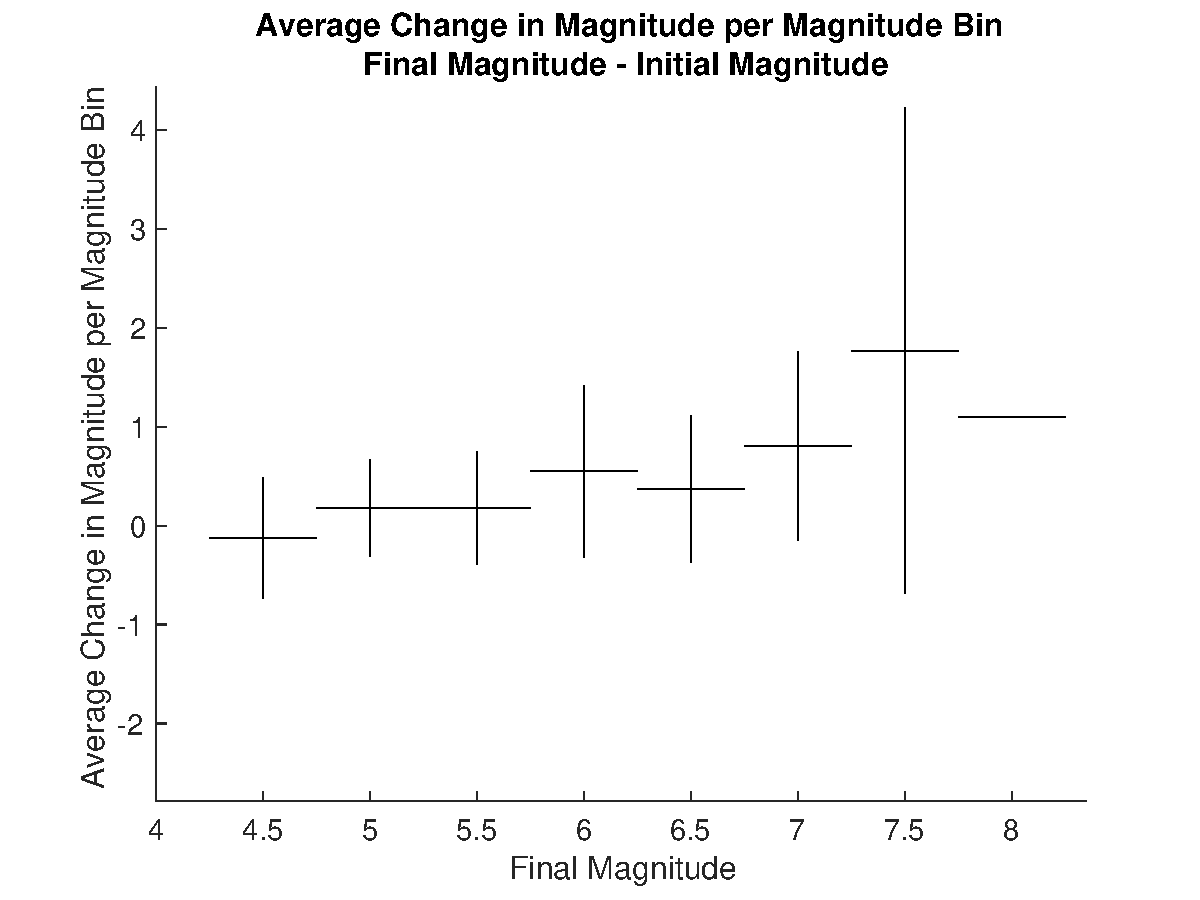
\includegraphics[trim = 0mm 0mm 1mm 0mm, clip = true, scale = 0.4]{plots/AverageChange.pdf}}
\end{figure}
\end{center}
\end{frame}

\begin{frame}
  \frametitle{Time delay - initiation of fault rupture and generation of the PDL client notification.}
\begin{center}
\begin{figure}[hbtp!]
  \subfigure[Time delay - initiation of fault rupture and generation of the PDL client notification.]{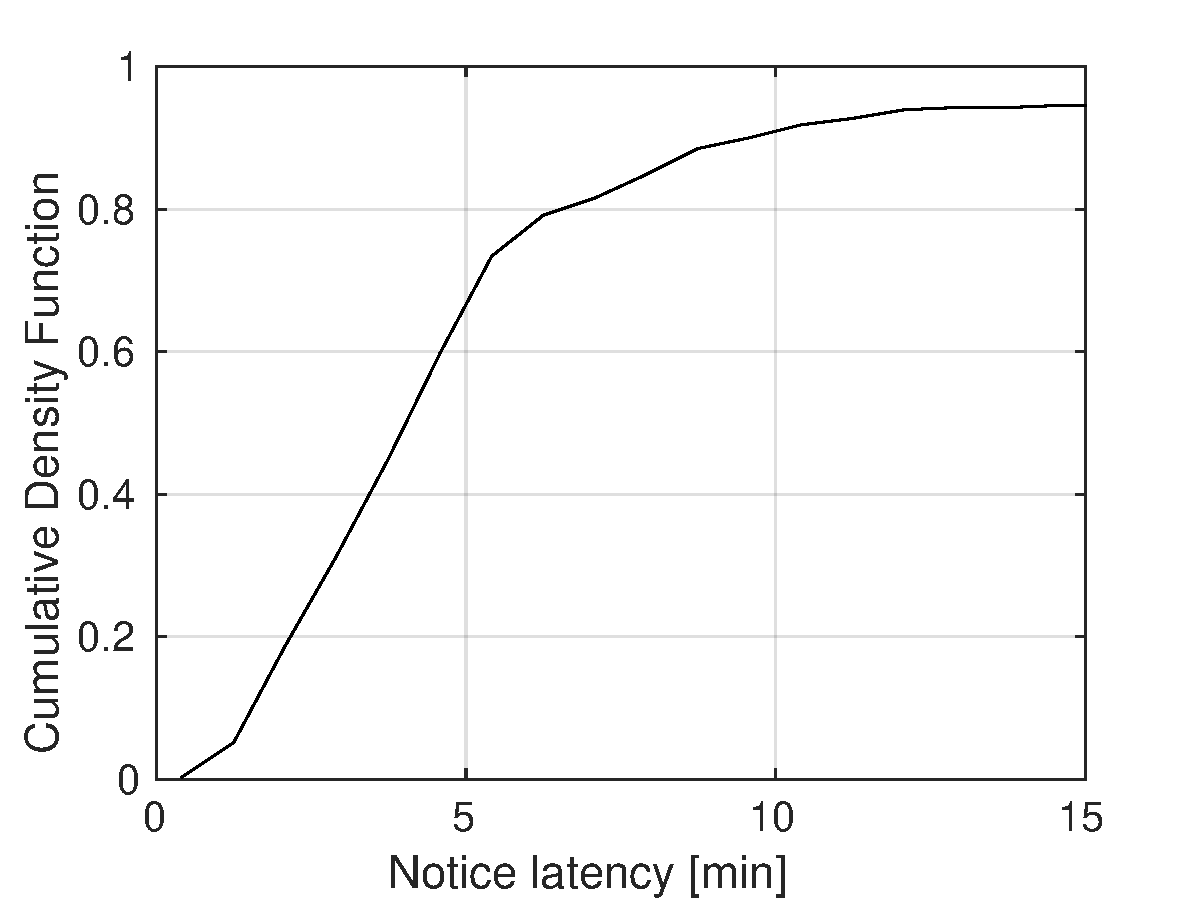
\includegraphics[trim = 0mm 0mm 1mm 0mm, clip = true, scale = 0.4]{plots/earthquake_notice.pdf}}
\end{figure}
\end{center}
\end{frame}

\begin{frame}
  \frametitle{Time delay - generation of the PDL client notification and surface wave arrivals.}
\begin{center}
\begin{figure}[hbtp!]
  \subfigure[Time delay - generation of the PDL client notification and surface wave arrivals.]{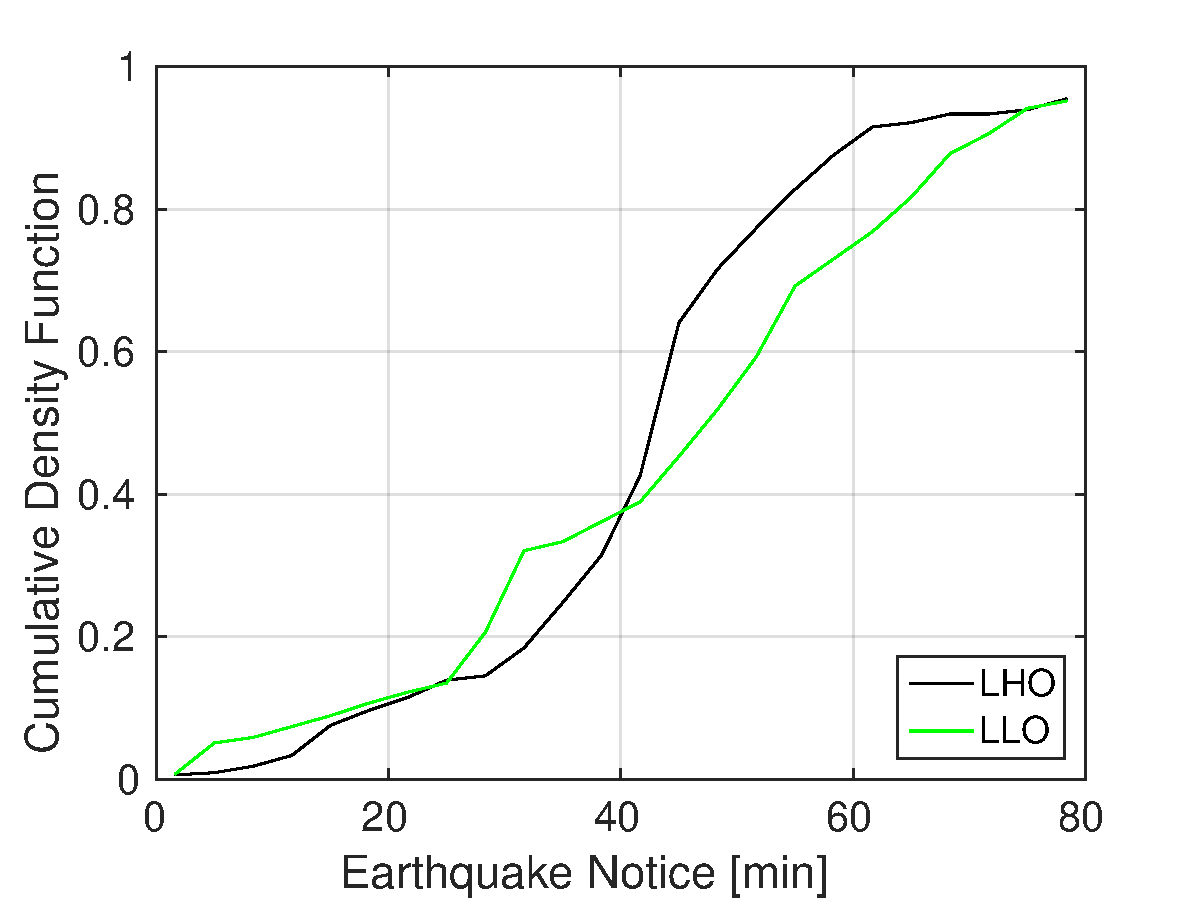
\includegraphics[trim = 0mm 0mm 1mm 0mm, clip = true, scale = 0.4]{plots/lockloss_notice.pdf}}
\end{figure}
\end{center}
\end{frame}

\begin{frame}
  \frametitle{Time of arrivals}
\begin{center}
\begin{figure}[hbtp!]
  \subfigure[Time of arrivals]{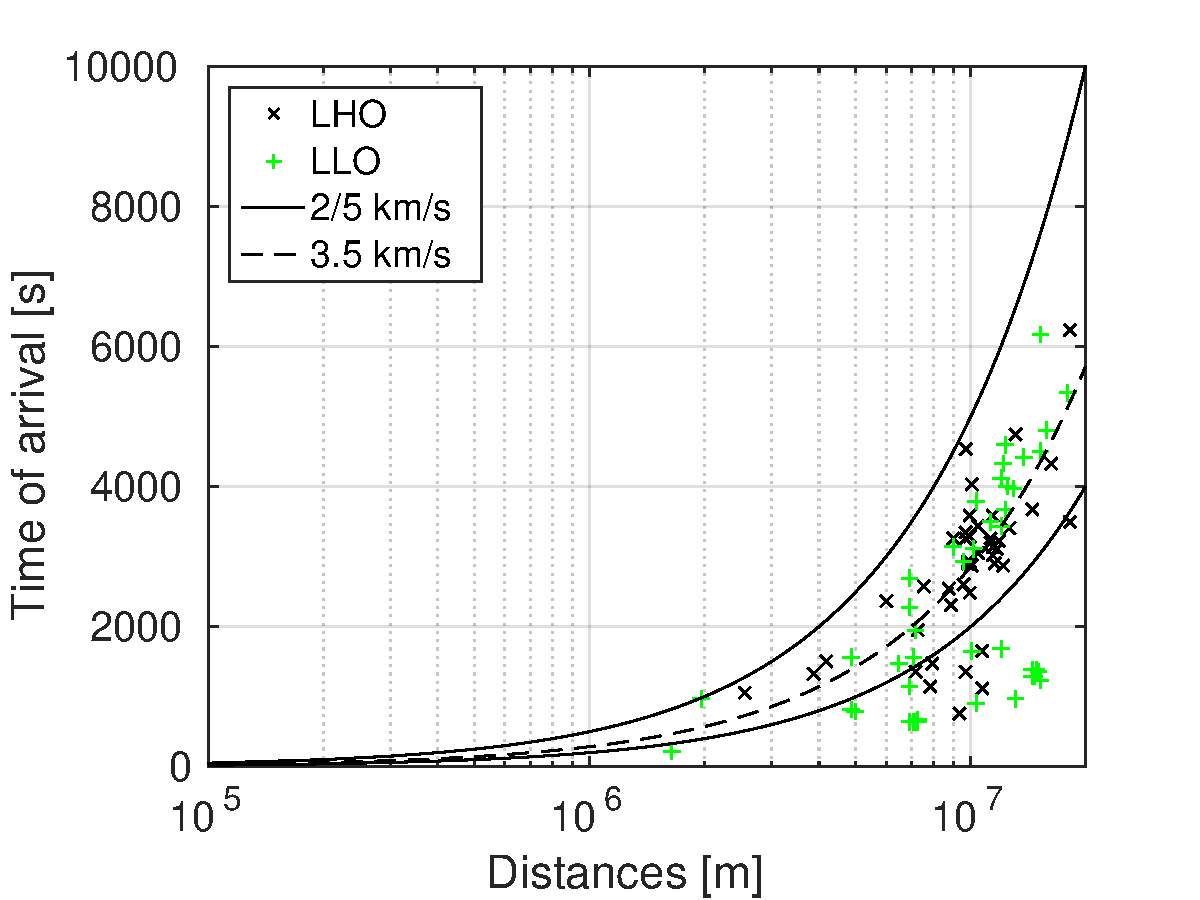
\includegraphics[trim = 0mm 0mm 1mm 0mm, clip = true, scale = 0.4]{plots/TOA.pdf}}
\end{figure}
\end{center}
\end{frame}

\begin{frame}
  \frametitle{Fit of peak velocities (LHO)}
\begin{center}
\begin{figure}[hbtp!]
  \subfigure[Fit of peak velocities (LHO)]{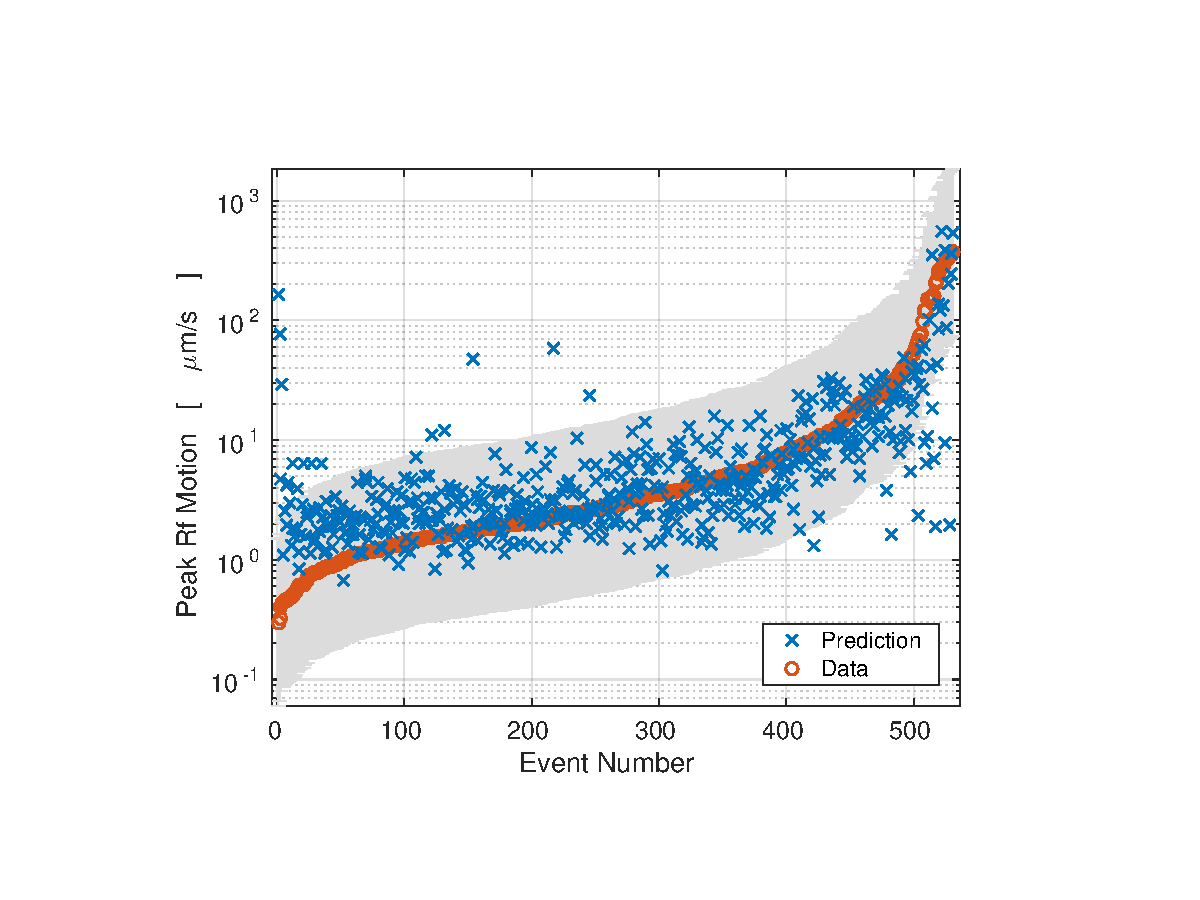
\includegraphics[trim = 0mm 0mm 1mm 0mm, clip = true, scale = 0.4]{plots/Prediction_LHO_S5_S6.pdf}}
\end{figure}
\end{center}
\end{frame}

\begin{frame}
  \frametitle{Fit of peak velocities (LLO)}
\begin{center}
\begin{figure}[hbtp!]
  \subfigure[Fit of peak velocities (LLO)]{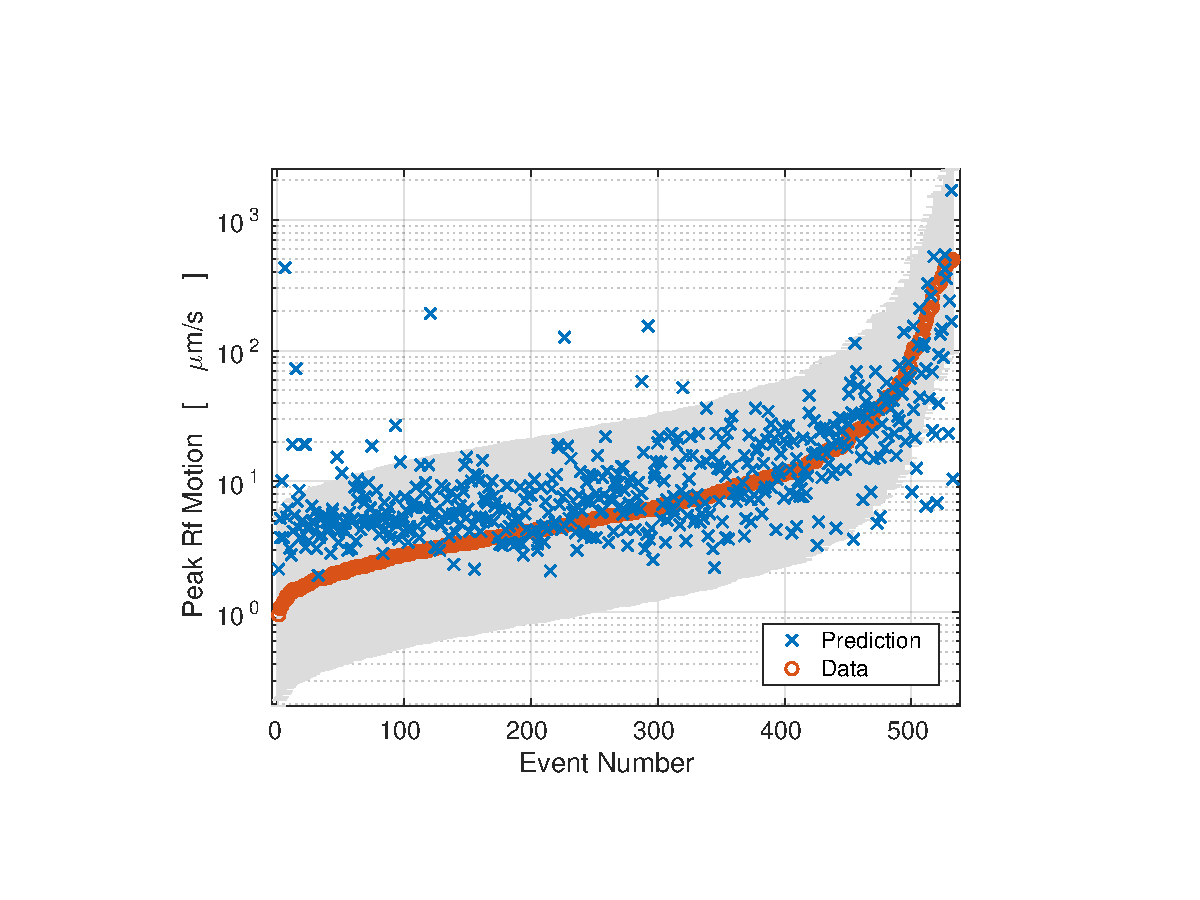
\includegraphics[trim = 0mm 0mm 1mm 0mm, clip = true, scale = 0.4]{plots/Prediction_LLO_S5_S6.pdf}}
\end{figure}
\end{center}
\end{frame}

\begin{frame}
  \frametitle{Predicted peak ground velocity as a function of magnitude}
\begin{center}
\begin{figure}[hbtp!]
  \subfigure[Predicted peak ground velocity as a function of magnitude]{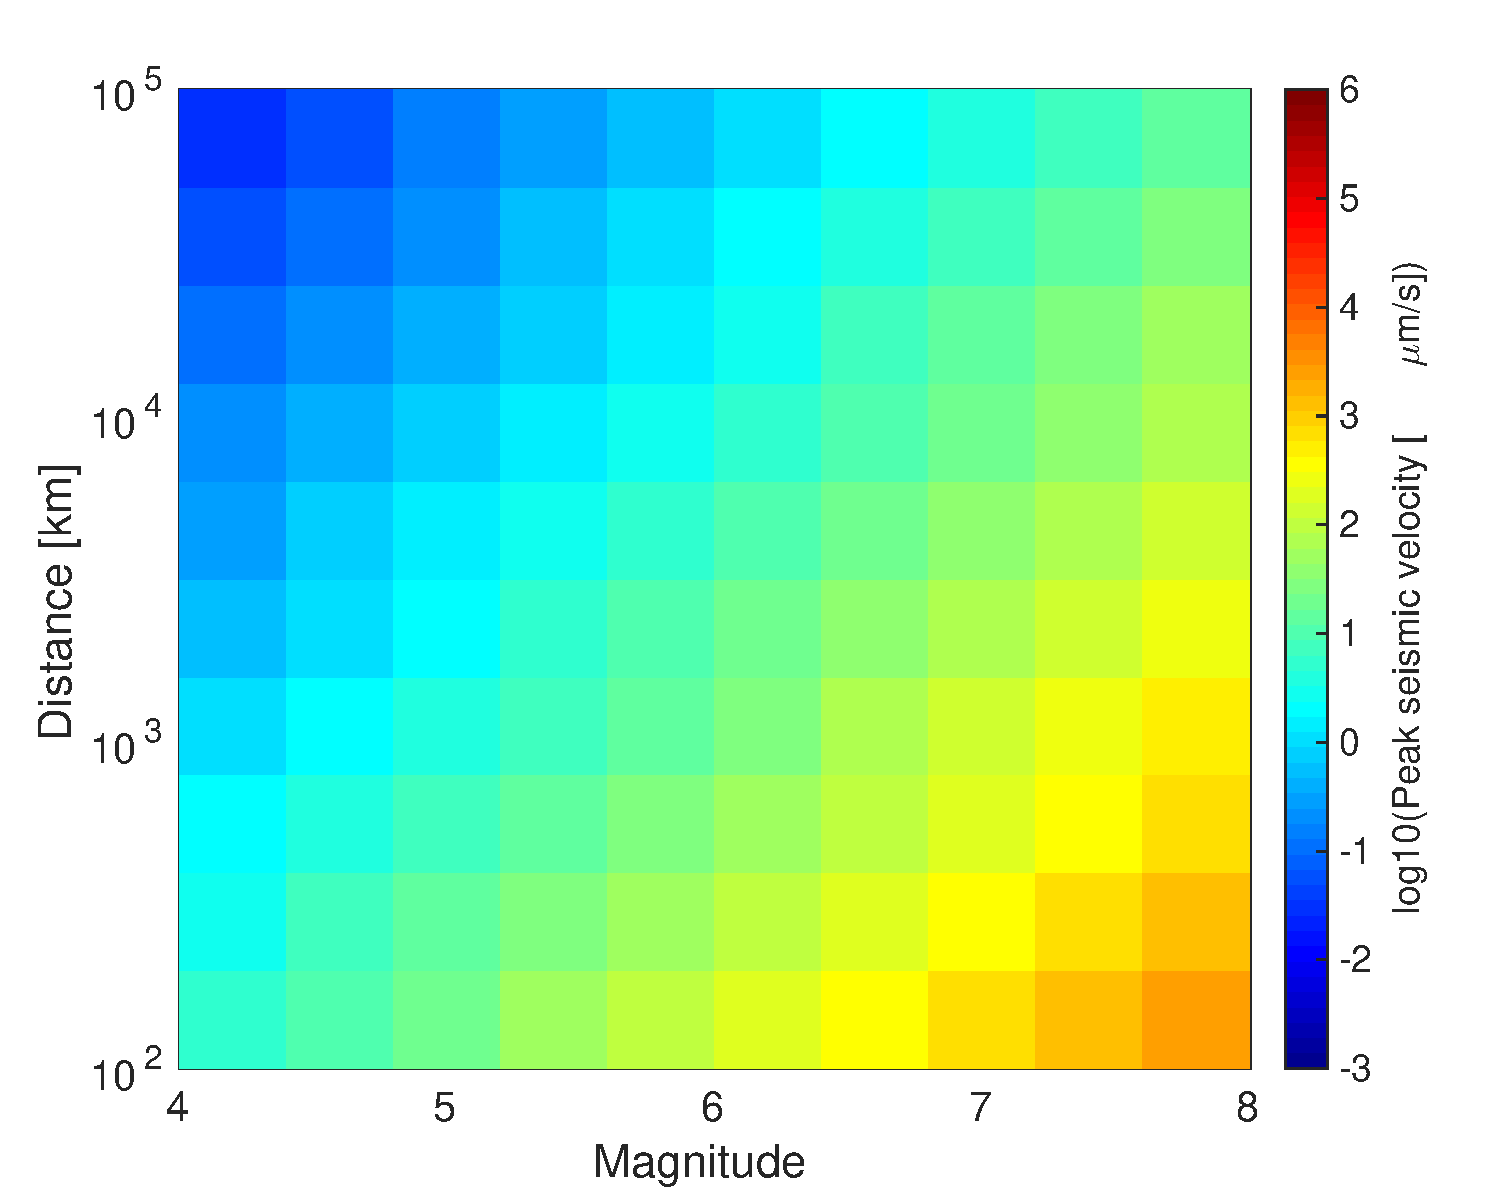
\includegraphics[trim = 0mm 0mm 1mm 0mm, clip = true, scale = 0.3]{plots/LHO_M_r.pdf}}
\end{figure}
\end{center}
\end{frame}

\begin{frame}
  \frametitle{Performance of estimation of peak velocities seen during O1 at the interferometers}
\begin{center}
\begin{figure}[hbtp!]
  \subfigure[Performance of estimation of peak velocities seen during O1 at the interferometers]{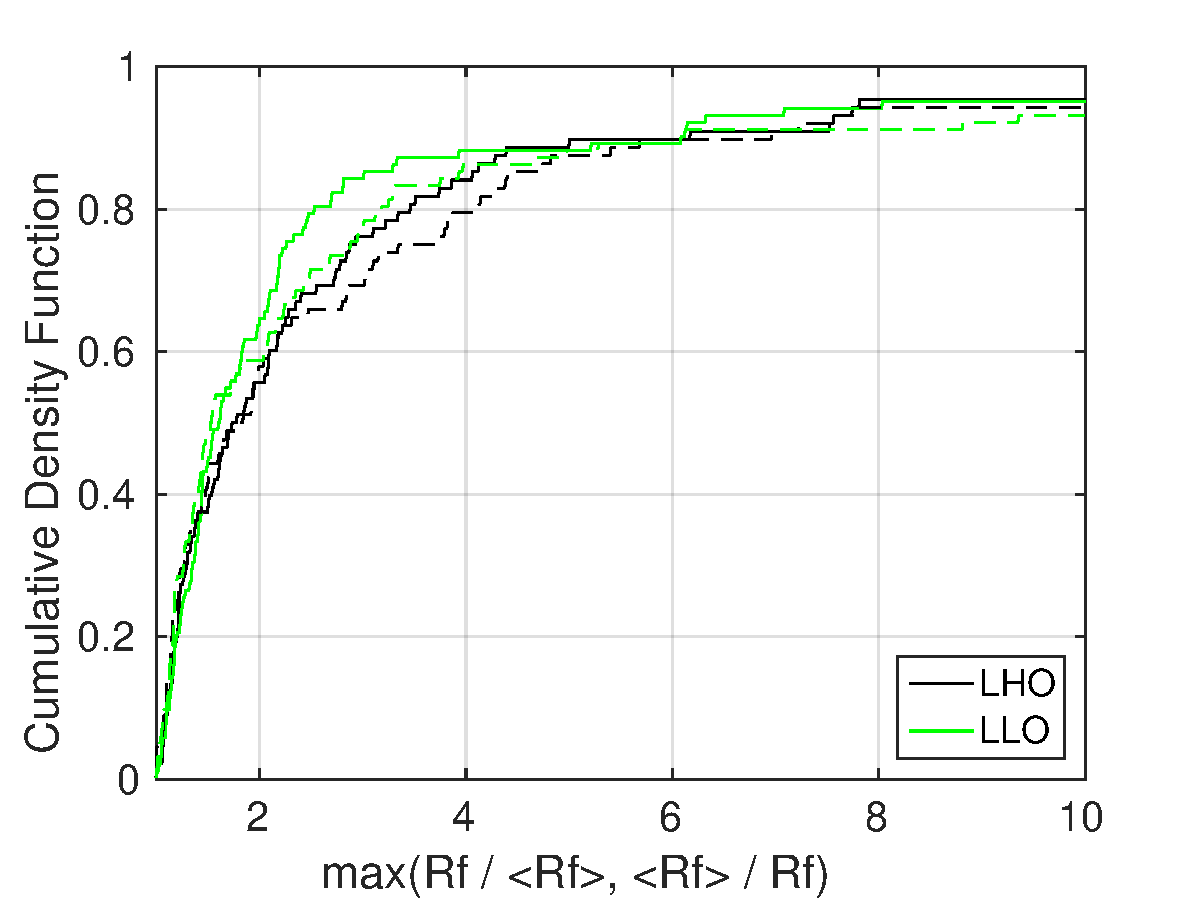
\includegraphics[trim = 0mm 0mm 1mm 0mm, clip = true, scale = 0.4]{plots/initial_final_vs_real.pdf}}
\end{figure}
\end{center}
\end{frame}

\begin{frame}
  \frametitle{Difference between the initial and final estimates of the earthquake time}
\begin{center}
\begin{figure}[hbtp!]
  \subfigure[Difference between the initial and final estimates of the earthquake time.]{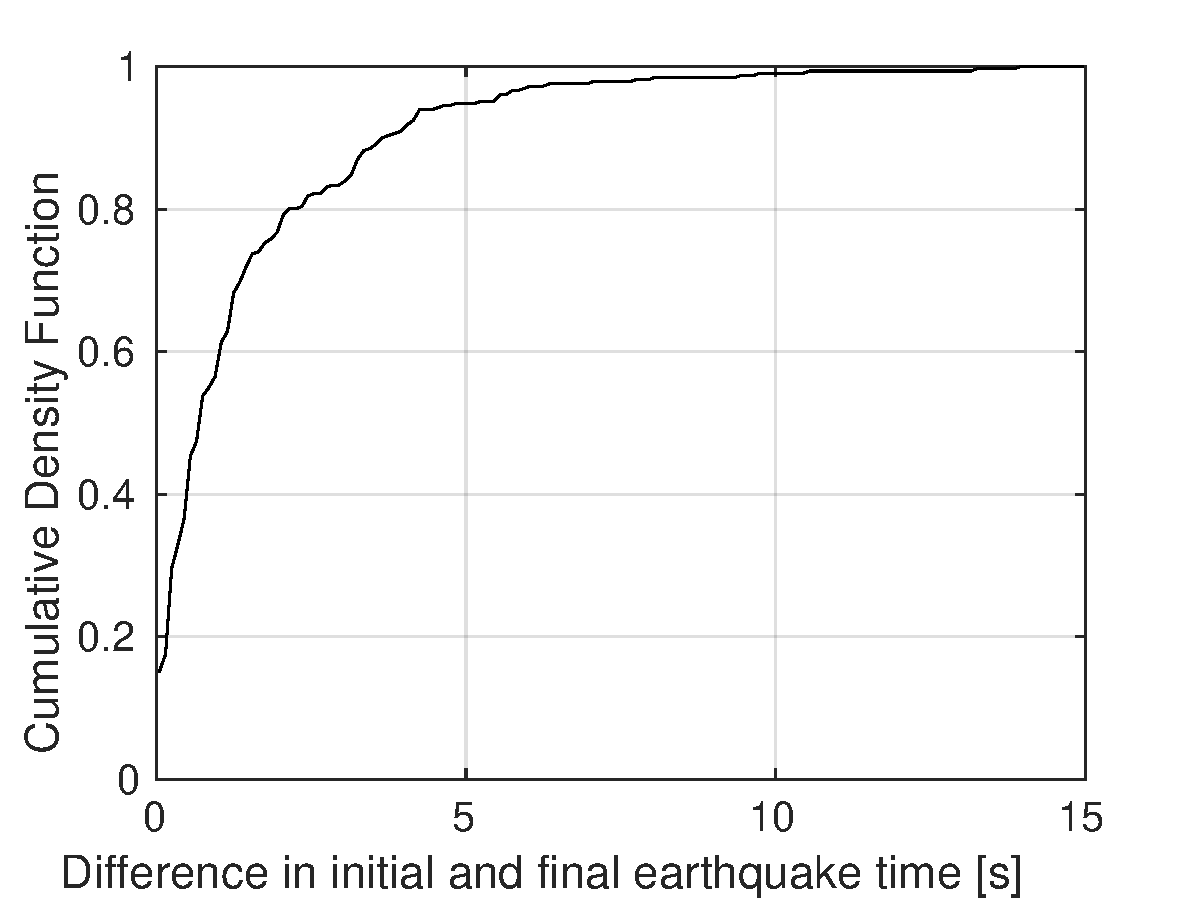
\includegraphics[trim = 0mm 0mm 1mm 0mm, clip = true, scale = 0.4]{plots/lockloss_est_timediff.pdf}}
\end{figure}
\end{center}
\end{frame}

\begin{frame}
  \frametitle{Lockloss as a function of predicted peak velocity vs. earthquake distance (LHO)}
\begin{center}
\begin{figure}[hbtp!]
  \subfigure[Lockloss as a function of predicted peak velocity vs. earthquake distance (LHO)]{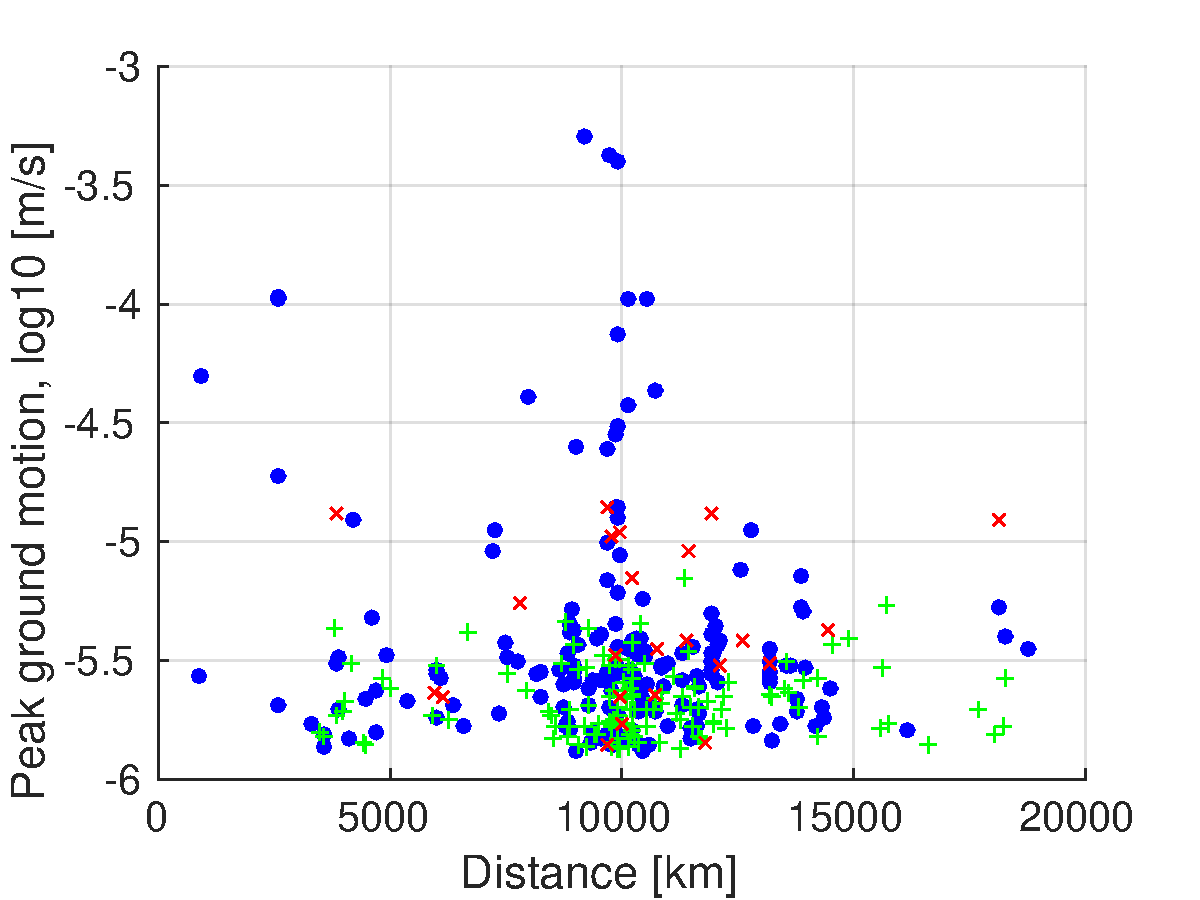
\includegraphics[trim = 0mm 0mm 1mm 0mm, clip = true, scale = 0.4]{plots/lockloss_vel_distance_LHO.pdf}}
\end{figure}
\end{center}
\end{frame}

\begin{frame}
  \frametitle{Lockloss as a function of predicted peak velocity vs. earthquake distance (LLO)}
\begin{center}
\begin{figure}[hbtp!]
  \subfigure[Lockloss as a function of predicted peak velocity vs. earthquake distance (LLO)]{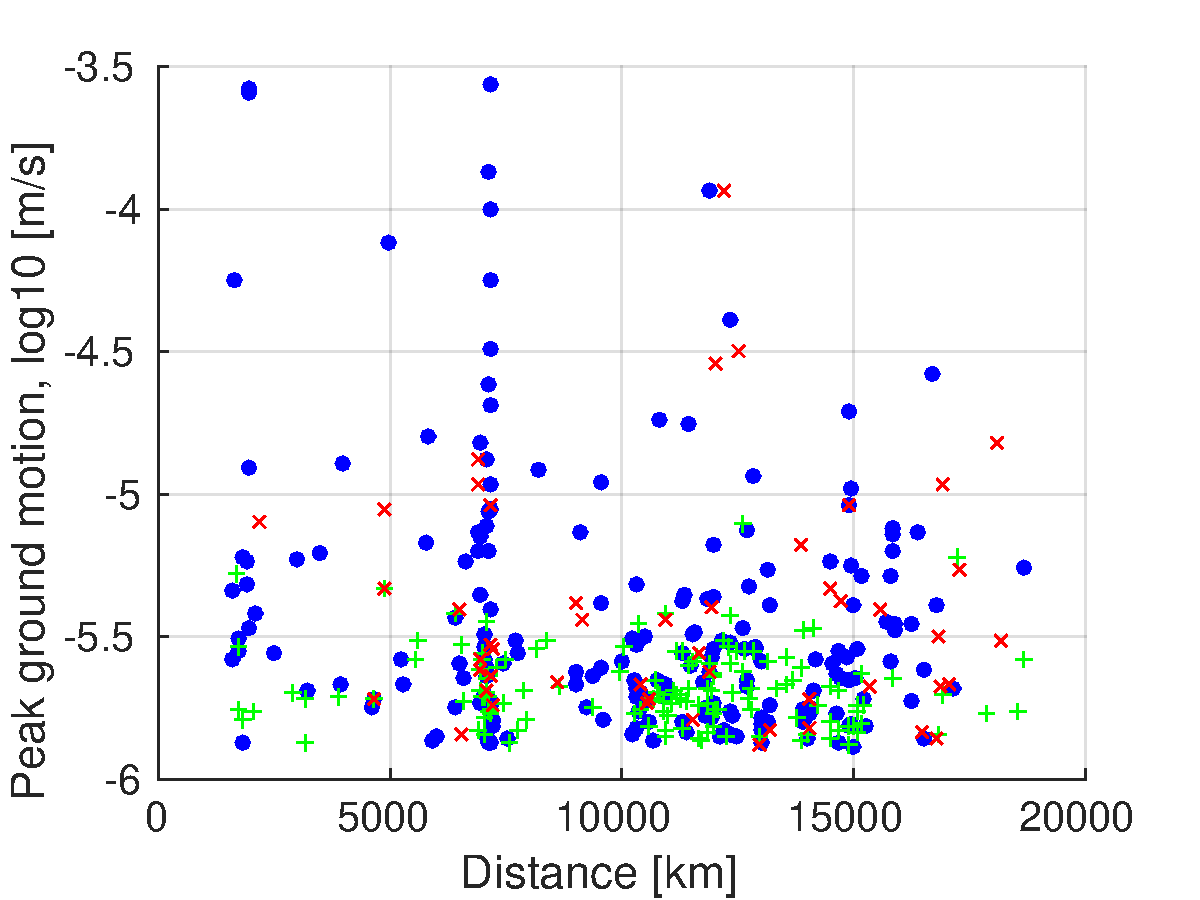
\includegraphics[trim = 0mm 0mm 1mm 0mm, clip = true, scale = 0.4]{plots/lockloss_vel_distance_LLO.pdf}}
\end{figure}
\end{center}
\end{frame}

\begin{frame}
  \frametitle{Performance of different machine learning classifier (LHO)}
\begin{center}
\begin{figure}[hbtp!]
  \subfigure[Performance comparison of different machine learning classifiers (LHO)]{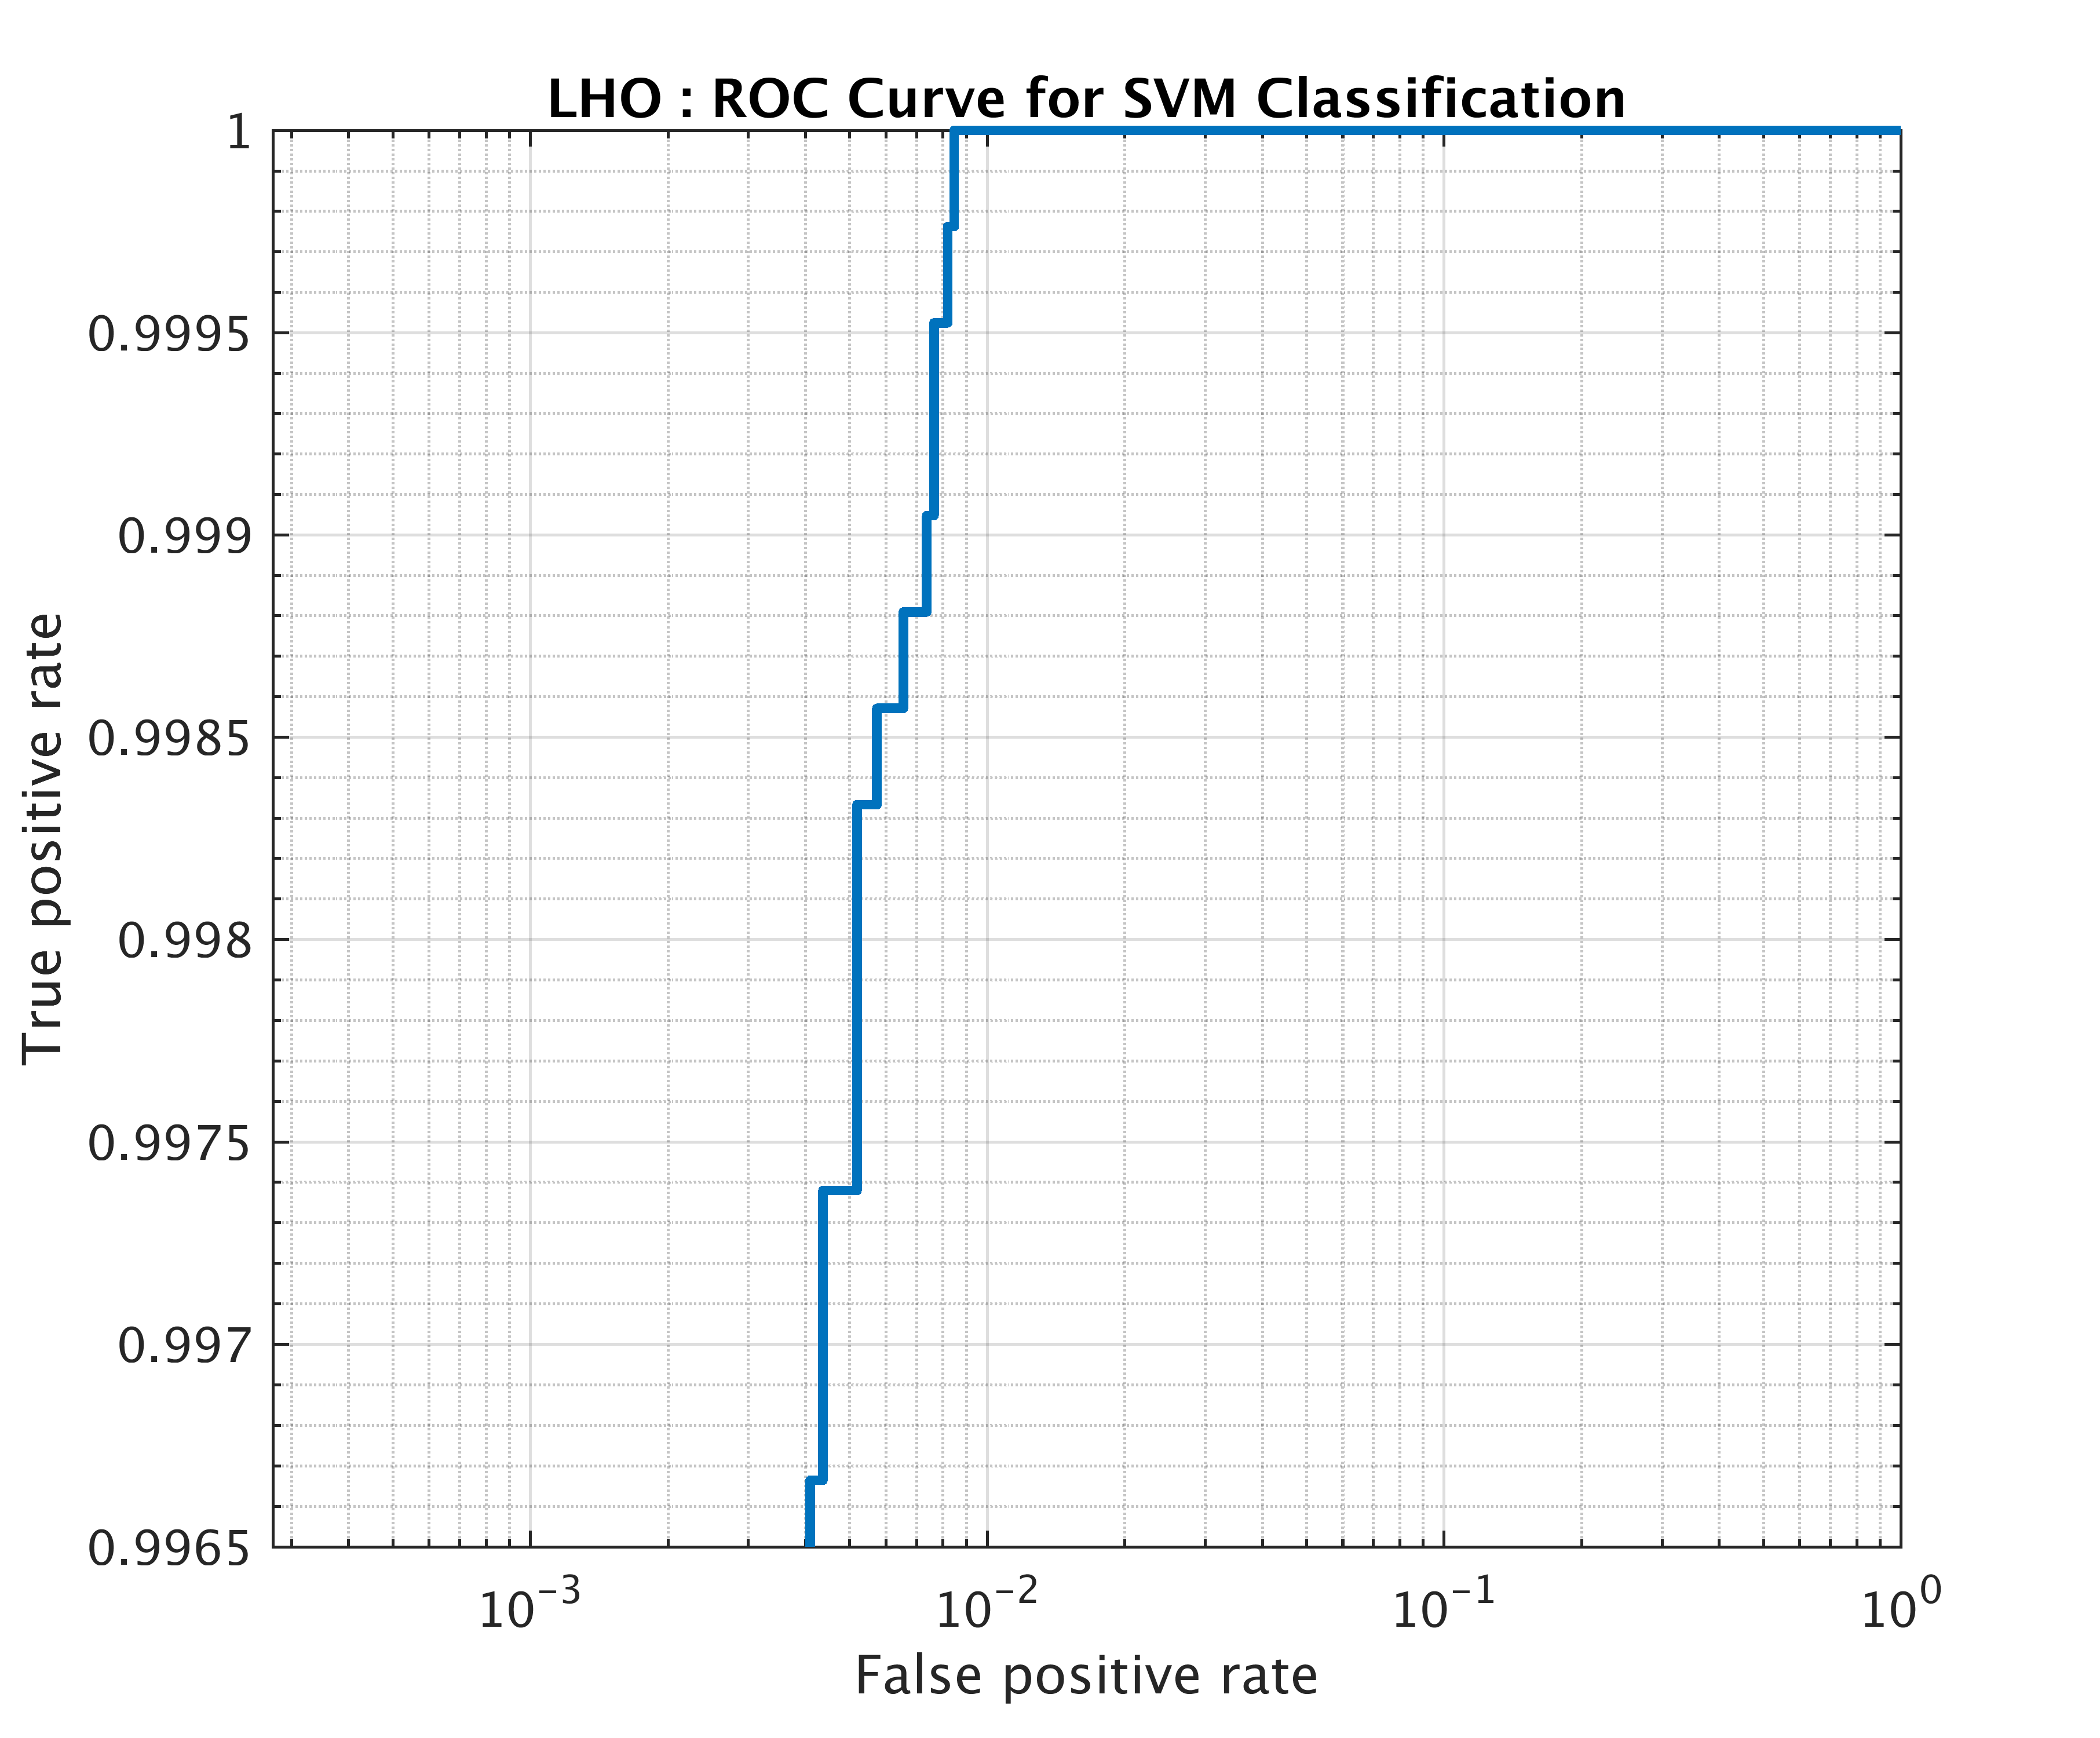
\includegraphics[trim = 0mm 0mm 1mm 0mm, clip = true, scale = 0.4]{plots/LHO_ROC_Optimized_SVM_loglog.png}}
\end{figure}
\end{center}
\end{frame}

\begin{frame}
  \frametitle{Performance of different machine learning classifier (LLO)}
\begin{center}
\begin{figure}[hbtp!]
  \subfigure[Performance comparison of different machine learning classifiers (LLO)]{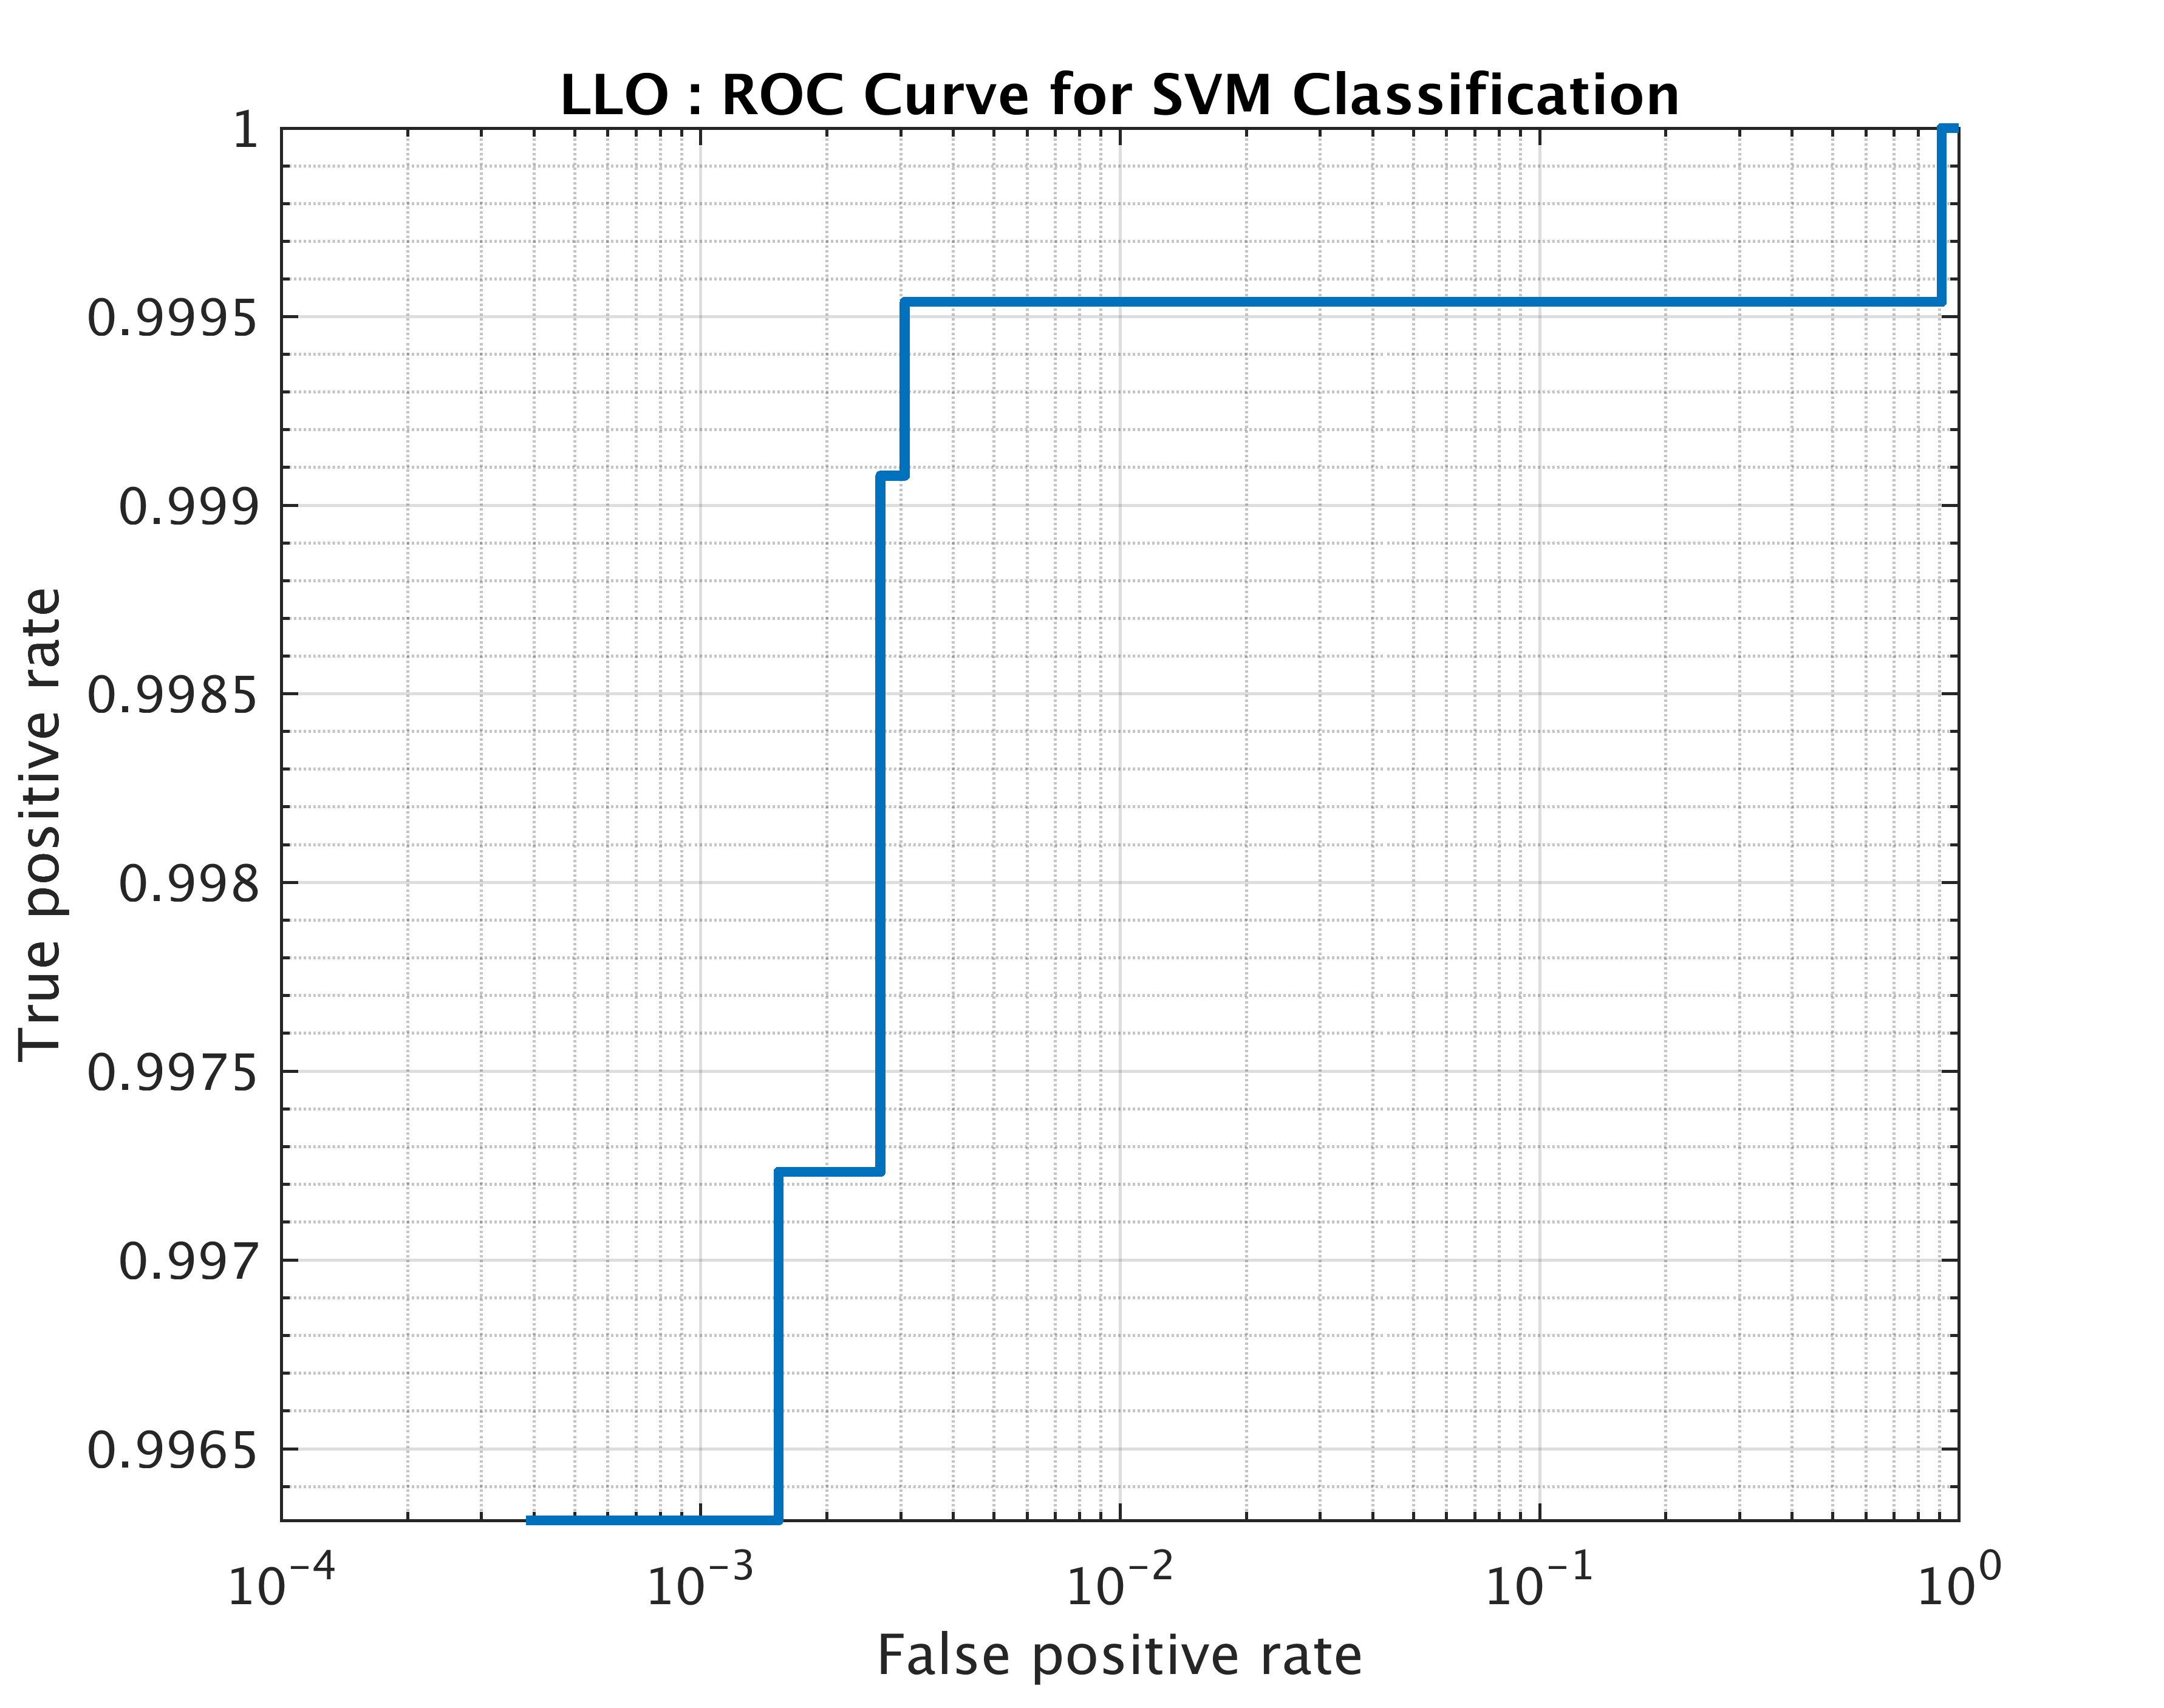
\includegraphics[trim = 0mm 0mm 1mm 0mm, clip = true, scale = 0.4]{plots/LLO_ROC_Optimized_SVM_loglog.png}}
\end{figure}
\end{center}
\end{frame}

\section{Conclusion}
\begin{frame}
  \frametitle{Current Status}

\begin{enumerate}
\item \emph{Seismon} is running reasonably well at LHO/LLO, with inputs to EPICs channels and the like. 
\item Currently using any earthquakes that come as tests by keeping the configuration the same and seeing what happens. Keith Thorne at LLO and Dave Barker at LHO are maintaining the codes there.
\item Virgo has installed and is running the code, and there is some debate about how to best use the output there.
\end{enumerate}

\end{frame}

\begin{frame}
  \frametitle{To-Do List}

There is much to do going forward ...
\begin{enumerate}
\item Updated amplitude fits using O1-O2 data. There is also the idea of using available IRIS data to make global fits, we have files containing 2015-2016 data for this that are being looked at.
\item Code or function for lockloss probability calculation
\item Generating lists of lock state (to do better than just locked vs. not locked) as we use in our current analysis.
\item Understanding what frequency band we most care about for lockloss (the seismic modeling community needs more information than just the broadband which we use for our empirical analysis)
\item Control configuration changes
\end{enumerate}

\end{frame}

\section{Extra slides}

\end{document}
